\documentclass[hyperref={pdfpagelabels=false}]{beamer}
\setbeamercolor{background canvas}{bg=white}
\usepackage{graphicx,lmodern,subfigure,ulem,color,graphicx,tikz,booktabs,natbib}
\usepackage{mathrsfs}
\usetheme{Warsaw}
%\definecolor{beamer@blendedblue}{rgb}{0.1,0.5,0.1}
%\definecolor{ForestGreen}{RGB}{60, 140, 60}
%\setbeamercolor{structure}{fg=beamer@blendedblue}
\setbeamertemplate{navigation symbols}{}
\setbeamertemplate{footline}[frame number]
\bibliographystyle{chicago}
\newcommand{\spitem}{\vspace{.3cm}\item}
\newcommand{\elas}{$E_{labor}$}
\def \ourFigPath {../../} 

\usetheme[
outer/progressbar=foot,
outer/numbering=none
]{metropolis}



\title{Sentiment Booms Go Wrong}
\author{Marco Brianti\\Vito Cormun}
\institute{Dissertation Workshop, Boston College}
\date{March 2019}


\begin{document}
	
	\frame{
		
		
		\maketitle
}



\frame{\frametitle{Two long Traditions in Macroeconomics}
	
	
	\bigskip
	
	\begin{enumerate}
		\item \textbf{Changes in expectation} as an important driver of economic fluctuations
		\begin{itemize}
			\item Incentives to anticipate future economic conditions.
			\begin{itemize}
				\item[$\Rightarrow$] Pigou (1927); Keynes (1936)
				\item[$\Rightarrow$] Beaudry and Portier (2004, 2006)
			\end{itemize}
			\end{itemize}
		
		%Changes in expectation may be an important independent element driving economic fluctuations. Agents have incentives to continuously anticipate the economy's future demands. If many agents adopt similar behavior because they receive related news about future developments, this will lead to a boom period. The idea of business cycles driven by expectations can be traced back to writing such as that of Pigou (1927), where he states, "The varying expectations of business men . . . constitute the immediate cause and direct causes	or antecedents of industrial fluctuations." According to Pigou, the very source of fluctuations is the "wave-like swings in the mind of the business world between errors of optimism and errors of pessimism." This view is also closely related to Keynes’ 1936 notion of animal spirits as it relates to these waves of optimism and pessimism as important driving forces behind economic fluctuations.
		
		%“Pigouvian” hypothesis that good news about the future may cause business cycle expansions - which in turn are reversed by less favorable news - has again become the subject of an important discussion within macroeconomics, due in large part to the pioneering work of Beaudry and Portier (2004, 2006)
		
		\
		
		\
		
		\item \textbf{Endogenous cycle}: expansions lead recessions
		\begin{itemize}
			\item Economic fluctuations are driven by \textbf{internal forces} which favor recurrent periods of boom and bust. 
			% Which this internal forces, well it depends on the model you have in mind and in the literature you focus on. For example the Austrian school of economics related to hayek and von Mises view recession and expansions of two faces of the same coin. During expansion the economy necesserily overaccumulate inputs which eventually has to liquidate during a recession. This last view as been revived by two different papers by BGP...
			%Alternatively, Minsky 1977 is more related to this excess optimism on the financial market, possibly related to either bounded rationality or financial frictions, which increase financial fragility in the economy and eventually lead to a bust. This view as been taken by Bordalo, Gennaioli, Shleifer (2018) which use a form of bounded rarionality (diagnostic expectation) to rationalize some boom-and-bust of the financial markets. "credit booms create risks to future macroeconomic performance, LopezSalido et al."
			\begin{itemize}
				\item[$\Rightarrow$] von Mises (1940); Beaudry, Galizia, and Portier (2018, 2019) %Austrian School, Hayek
				\item[$\Rightarrow$] Minsky (1977); Bordalo, Gennaioli, Shleifer (2018) %{Euphoria} leads to excessive credit and higher financial fragility 
			\end{itemize}
			\end{itemize}
		
	%	\
		
		%\item \textbf{Excessive optimism} eventually leads to a recession
	%	\begin{itemize}
		%	\item \textbf{Unrealized expectations} on future fundamentals 
		%	\begin{itemize}
		%		\item[$\Rightarrow$] Pigou, 1927; Beaudry and Portier, 2004
		%	\end{itemize}
		%	\item \textbf{Over-accumulation} during booms 
		%	\begin{itemize}
		%		\item[$\Rightarrow$] von Mises, 1940; Beaudry, Galizia, and Portier, 2018
		%	\end{itemize}
		%	\item \textbf{Euphoria} leads to excessive credit and higher financial fragility 
		%	\begin{itemize}
			%\item[$\Rightarrow$] Minsky, 1977; Bordalo, Gennaioli, Shleifer, 2018 
			%\end{itemize}
		%\end{itemize}
		%1. Pigou (1926), when agents are optimistic about the future and decide to build up capital in expectation of future demand then, in the case where their expectations are not met, there will be a period of retrenched investment which is likely to cause a recession.
		%The notion of optimism simply refers to a state where agents receive an above average signal. In this environment, periodic recessions are most likely to arise when agents signals about the future are precise. In effect, in our framework, occasional recessions are a sign of a well-functioning economy since they reflect the availability of good quality information upon which	people act.
		%According to Hayek, recessions mainly reflect periods of liquidation resulting from past over-accumulation of capital goods. A situation where the economy needs to liquidate such an excess can quite naturally give rise to a recession. As suggested by Hayek, such a situation can readily lead to a recession as less economic activity is generally warranted when agents want to deplete past over-accumulation. 
		%One potential criticism of a pure liquidationist view of recessions is that, if markets functioned efficiently, such periods should not be very socially painful. In particular, if economic agents interact in perfect markets and realize they have over-accumulated in the past, this should lead them to enjoy a sort of holiday paid for by their past excessive work. In contrast, in our environment we will show that liquidation periods are generally socially painful because of the multiplier process induced by cautious spending and unemployment risk. The force that links the markets is precautionary behavior. Once there is less demand in the durable goods sector, agents fearing unemployment reduce demand in both sectors, thereby causing the decreased demand in the durable sector to spillover into non-durables.
		

		%According to an old argument (e.g., Minsky 1977), investor optimism brings about the expansion of credit and investment, and leads to a crisis when such optimism abates.  
		%New York Times' article: There are basically five stages in Minsky’s model of the credit cycle: displacement, boom, euphoria, profit taking, and panic.  A displacement occurs when investors get excited about something —an invention, such as the Internet, or a war, or an abrupt change of economic policy.  With the cost of borrowing at historic lows, a speculative real-estate boom quickly developed. As a boom leads to euphoria, banks and other commercial lenders extend credit to ever more dubious borrowers.
	\end{enumerate}
	

}


\frame{\frametitle{This paper}
	
\begin{enumerate}
	\item We empirically estimate \textbf{sentiment shocks} and evaluate their effects on aggregate U.S. variables
	\begin{itemize}
		\item We define sentiment shocks as \textbf{changes in expectations} uncorrelated with fundamentals		
		\item Sentiment shocks trigger \textbf{boom-and-bust dynamics} on most macroeconomic variables
		\item Sentiments explain up to \textbf{40\% of output} 
	\end{itemize}
	
	\
	
	\
	
	\item We write a \textbf{general equilibrium model} that rationalizes our empirical findings
	\begin{itemize}
		\item 			
		\item 
	\end{itemize}
\end{enumerate}

}


\frame{\frametitle{Contributions}
	
	

\begin{enumerate}
	\item \small{We use Instrumental Variable Local Projection (\textbf{IV-LP}) to estimate sentiments shocks}
	\begin{itemize}
		\item \footnotesize{Previous literature estimates DSGE models or employ SVAR}
		\begin{itemize}
			\item[$\Rightarrow$] Milani, 2011; Levchenko and Pandalai-Nayar, 2018
		\end{itemize}
	\end{itemize}
		
		%Milani (2011, EJ): This article evaluates the empirical role of expectational shocks on business cycle fluctuations and relaxes the rational expectations assumption to exploit survey data on expectations in the estimation of a New Keynesian model, which allows for learning by economic agents. Expectation shocks affect the formation of expectations and capture waves of optimism and pessimism that lead agents to form forecasts that deviate from those implied by their learning model.
        
        %Leduc and Sill (2013, RESTUT): VAR controlling for fiscal and oil shocks. They get the bust significant but they do not emphasize it.
        
        %Levchenko and Pandalai-Nayar (2018, JEEA): they estimate the international transmission of three identified shocks—surprise TFP, news of future TFP, and sentiment. Sentiment shocks max output on impact after controlling for TFP and News. The US sentiment shock produces a business cycle in the United States, with output, hours, and consumption rising following a positive shock, and accounts for the bulk of the US short-run business cycle fluctuations.
        
        %Feve and Guay (2018, EJ): Sentiments shocks are identified as shocks orthogonal to fundamentals that account for most of the variance of confidence. We obtain that, contrary to news shocks on total factor productivity, sentiment shocks explain little of quantities and prices. Sentiments shocks mostly appear as an idiosyncratic component of confidence. These results are robust to various perturbations. (i) orthogonal to fundamentals (for example, expected and unexpected or surprise TFP shocks); (ii) with no long-run effect on TFP and other real quantities; and (iii) that accounts for most of the variance of various measures of confidence.

\bigskip

	\item Uncover \textbf{new dynamics} in response to sentiment shocks 
	\begin{itemize}
		\item \footnotesize{\textbf{Informative} for the literature on sentiments}
		\begin{itemize}
		\item[$\Rightarrow$] Angeletos and La'O, 2013; Angeletos et al. (2018)
		\end{itemize}
		
		%Angeletos and La'O (2013) limit communications among islands. They then show that the BC is driven by a certain type of extrinsic shocks which they call sentiments. These shocks formalize shifts in expectations of economic activity without shifts in the underlying preferences and technologies. They are akin to sunspot but operate in unique-equilibrium models.
		
		% They estimate their model on the frequency domain removing frequency below 6 quarters and above 32 quarters. They match a peak in the spectral density at about 28 quarters. Which is the same period of our estimated cycle.
		
		%Chahrour and Gaballo (2018) provide a new theory of expectations-driven business cycles based on learning from prices. Upon observing a price change, households are unsure about its cause: a price increase caused by lower productivity may be misinterpreted as an improvement in local conditions, leading households to consume more. As a result, unobserved productivity shocks generate positive price-quantity comovement. The feedback of beliefs into prices can be so strong that even arbitrarily-small surprises in productivity lead to substantial fluctuations

	
	% Self-fulfilling equilibria and indeterminacy can easily arise in a simple financial accelerator model with reasonable parameter calibrations and without increasing returnsin production. A key feature for generating indeterminacy in our model is the countercyclical markup due to the procyclical loan-to-outputratio. We illustrate, via simulations, that our financial accelerator model can generate rich business cycle dynamics, including hump-shaped output in response to demand shocks as well as autocorrelation in output growth rates.

		\end{itemize}
	
	\bigskip
	
	
	\item New supportive evidence for the literature on \textbf{credit cycles}
	\begin{itemize}
		\item \footnotesize{We proposed \textbf{structural evidence} in favor credit booms with negative macroeconomic consequences}
		\begin{itemize}
			\item[$\Rightarrow$] Lopez-Salido, Stein, and Zakrajsek (2017) 
			%Mian Sufi? Greenwood and Hanson? TO BE DISCUSSED
		\end{itemize}
		\end{itemize}
	

	
	\bigskip
	
	\item (Ideally) Theory that displays \textbf{boom-and-bust} dynamics conditional on a specific type of shock
	\begin{itemize}
		\item Hard to get shock specific boom and busts
		\begin{itemize}
			\item[$\Rightarrow$] Beaudry, Galizia, and Portier (2019)
		\end{itemize} 
		\end{itemize}
	
	% This paper explores a theory of business cycles in which recessions and booms arise due to difficulties encountered by agents ion properly forecasting the economy's future needs in terms of capital. They illustrate the type of general equilibrium structure that can give rise to such phenomena. 
	    
\end{enumerate}	
		
}

\frame{\frametitle{Roadmap}
	\large{
		$ \ \ \ \ \ \ \ $ 1. \textbf{Empirical Strategy}
		
		$ \ \ \ \ \ \ \ $ 2.  Empirical Results
		
		$ \ \ \ \ \ \ \ $ 3. Test
		
		$ \ \ \ \ \ \ \ $ 4. Model
		
		$ \ \ \ \ \ \ \ $ 5. Conclusions
	}
}




\frame{\frametitle{Econometric Strategy}
	
	A 2-step procedure:
	
	\bigskip
	
	\begin{enumerate}
		\item Build an \textbf{instrument} $Z_t$ correlated with changes in expectations and orthogonal to fundamentals.
		
		\bigskip
		
		\vskip 20pt
		
		\item Estimate \textbf{dynamic responses} of macroeconomic variables using IV-LP.
		
		\end{enumerate}
	



	
}

\frame{\frametitle{Data Treatment on Expectations}
	
	\bigskip 
	
	 Quarterly data from 1982 to 2018 of forecasts on macroeconomic variables, $X^s_t$, made by \textbf{Survey of Professional Forecasters} 
	
	\bigskip
	
	Define, 
	\begin{itemize}
		\item $E^i_t ( X^s_{t+k} )$ as the expectation on $X^s_{t+k}$ given the information set at time $t$ released by professional forecaster i
		
		\bigskip
		
		\item $E_t ( X^s_{t+k} )$ as the sample mean across $i$ of $E^i_t ( X^s_{t+k} )$
		
		\bigskip
		
		\item $E_t(\hat{x}_{t+k}^s) =  E_t ( X_{t+k}^s ) / E_t ( X_{t}^s )  - 1$ as the expectation of the growth rate of $X^s$ from $t$ to $t+k$ given information set $t$
		
		\bigskip
		
		\item $R_{t,k}^s =  E_t(\hat{x}_{t+k}^s) -  E_{t-1}(\hat{x}_{t+k}^s)$ as the revision on expectations from $t-1$ to $t$ of the growth rate of $X^s$ from $t$ to $t+k$
		%\begin{itemize}
			%\item due to data availability, $k = 1,2,3$.
		%\end{itemize}
	
	\bigskip
	
	\item $R_t^k$ is the first principal component of $R_{t,k}^s$
	\end{itemize}
	
	
	%\begin{eqnarray*}
	%E ( X_{t+k} |I_t) = \begin{bmatrix}
	%E ( \text{RGDP}_{t+k} |I_t) \\
	%E ( \text{NGDP}_{t+k} |I_t) \\
	%E ( \text{RI}_{t+k} |I_t) \\
	%E ( \text{RC}_{t+k} |I_t) \\
	%E ( \text{IP}_{t+k} |I_t) \\
   % \end{bmatrix}
%	\end{eqnarray*}


%to estimate forecast revisions on the growth rate of macroeconomic aggregates
	
	
	
}

\frame{\frametitle{IV-LP Estimator}
	
	\bigskip
	
	Dynamic response of endogenous variable $Y_{t+h}$ to $R_t$ is
	\begin{eqnarray}\label{endo_reg}
	Y_{t+h} = \Theta_{h}^Y R_t + u^Y_{h,t+h}
	\end{eqnarray}
	
	
	\bigskip
	
	Because $R_t$ is endogenous, OLS estimation of \ref{endo_reg} is not valid. Eq. \ref{endo_reg} can be estimated by IV if $Z_t$ satisfies the following conditions
	\begin{enumerate}
		\item $E(\varepsilon_{1,t}Z_t) = \alpha \neq 0$ (relevance)
		\item $E(\varepsilon_{2:N,t}Z_t) = 0$ (contemporaneous exogeneity)
		\item $E(\varepsilon_{1:N,t+j}Z_t) = 0$ for $j \neq 0$ (lead-lag exogeneity)
	\end{enumerate}
	
	%Condition LP-IV (iii) arises because of the dynamics. The key idea of this condition is that Y,t+h generally depends on the entire history of the shocks, so if Zt is to identify the effect of shock ɛ1,t alone, it must be uncorrelated with all shocks at all leads and lags. The requirement that Zt be uncorrelated with future e’s is generally not restrictive: when Zt contains only variables realised at date t or earlier, it follows from the definition of shocks as unanticipated structural disturbances. In contrast, the requirement that Zt be uncorrelated with past e’s is restrictive and strong. We will refer to Condition LP-IV (iii) as requiring that Zt be unpredictable given past e’s, although strictly the requirement is that it not be linearly predictable given past e’s. Note that Zt could be serially correlated yet satisfy this condition. For example, suppose Zt = dɛ1,t + ft, where ft is a serially correlated error that is independent of {et}; then Zt satisfies Condition LP-IV.
	
	Given the validity of previous conditions, a consistent estimator for $\Theta_h^Y$ is defined as
	\begin{eqnarray*}
	\widehat{\Theta}_h^Y = \frac{\sum_{t=0}^{T-h} Y_{t+h}Z_t}{\sum_{t=0}^{T-h}  R_t Z_t}
	\end{eqnarray*}
	
}


\frame{\frametitle{Instrument $Z_t$}
	
	
	\bigskip
	
	We estimate instrument $Z_t$ as the unpredictable component of $R_t$ orthogonal to fundamentals,
	\begin{eqnarray*}
	R_t = c + B(L) \Delta TFP_{t} + \delta W_t + Z_t
	\end{eqnarray*}
	
	where,
	\begin{itemize}
		\item $\Delta TFP$ is the first difference of utilization-adjusted TFP 
		\item $W_t$ represents a series of controls 
		\begin{itemize}
			\item Lagged principal components
			\item Other structural shocks
		\end{itemize}

	\end{itemize}

\

Importantly, R-Squared are relatively small (30\%-50\%)
\begin{itemize}
	\item[$\Rightarrow$] A large part of SPF expectations is unrelated to fundamentals
	\item[$\Rightarrow$] $Z_t$ is a relevant instrument
\end{itemize}
	
	
}







\frame{\frametitle{Roadmap}
	\large{
		$ \ \ \ \ \ \ \ $ 1. Empirical Strategy
		
		$ \ \ \ \ \ \ \ $ 2.  \textbf{Empirical Results}
		
		$ \ \ \ \ \ \ \ $ 3. Test
		
		$ \ \ \ \ \ \ \ $ 4. Model
		
		$ \ \ \ \ \ \ \ $ 5. Conclusions
	}
}


\frame{\frametitle{Impulse Responses (I)}
	
	\bigskip
	
	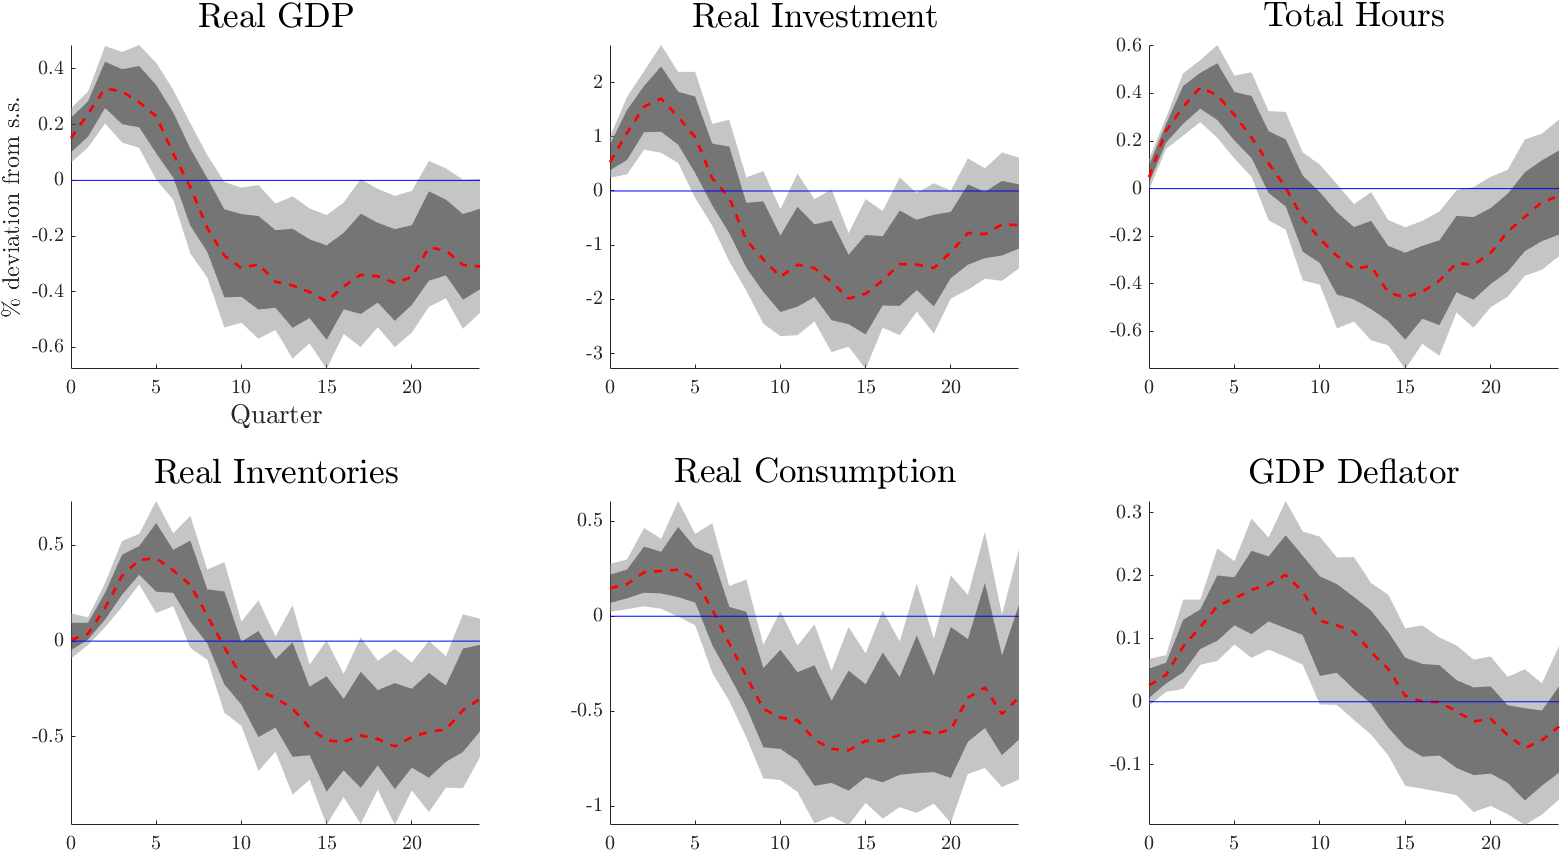
\includegraphics[scale=0.26]{main_IRFs}
	
}


\frame{\frametitle{Impulse Responses (I)}
	
	\bigskip
	
	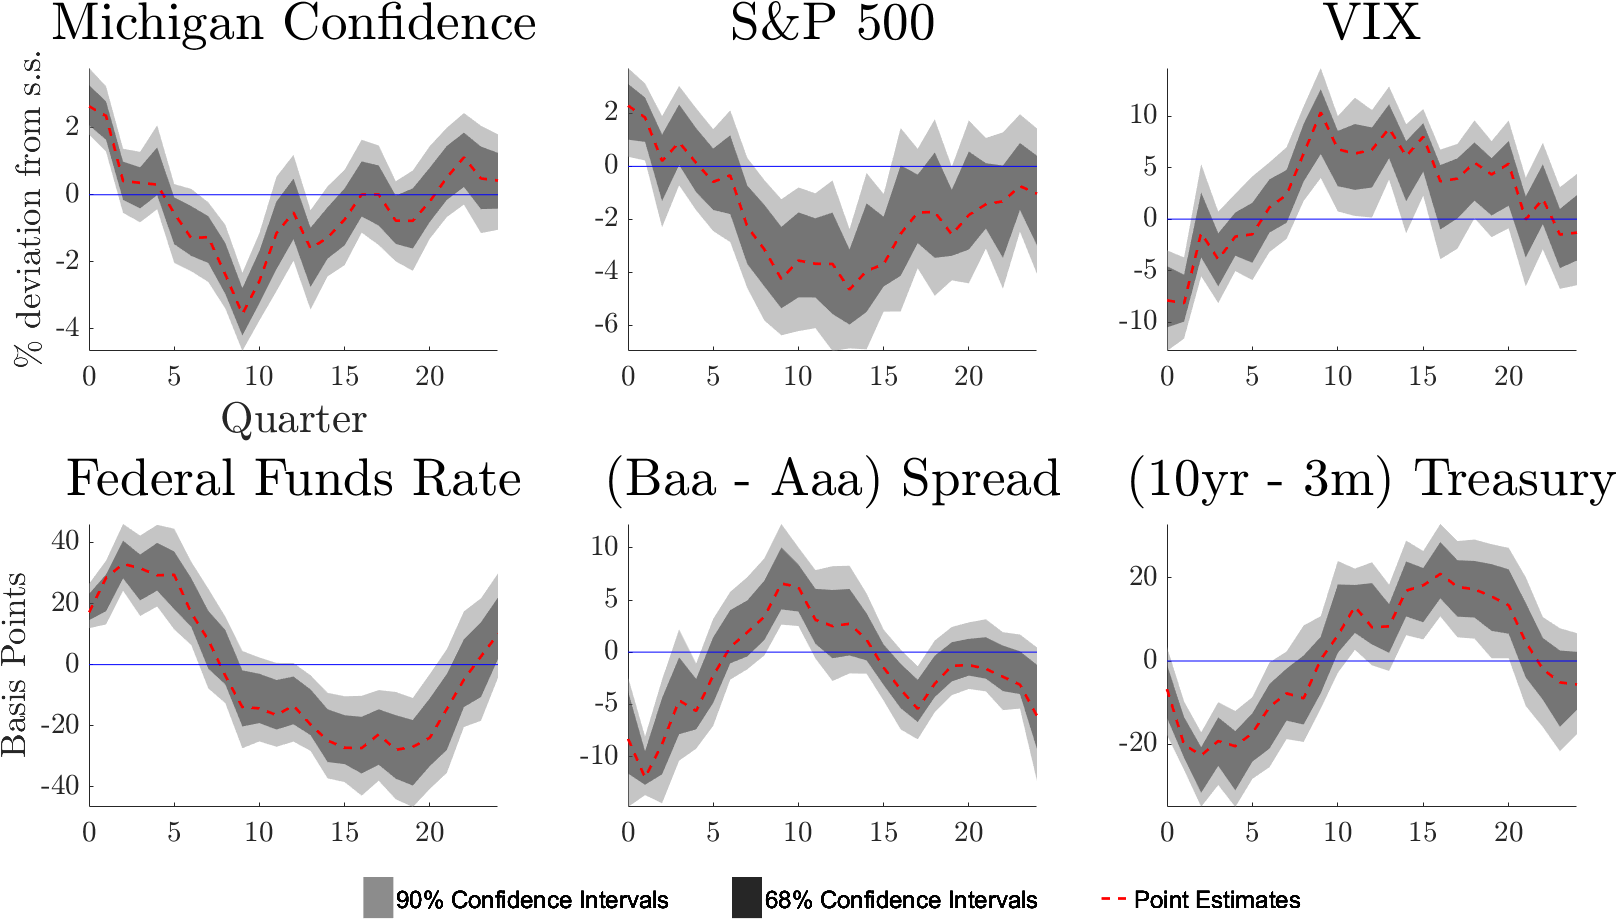
\includegraphics[scale=0.26]{additional_IRFs}
	
}

\frame{\frametitle{Variance Decomposition}
	
\begin{table}[]
	\begin{tabular}{r|cccc}
		& \textit{Impact} & \textit{1 Year} & \textit{2 Years} & \textit{5 Years} \\ \hline
Real GDP		    & 9.38\%       & 19.81\% & 16.50\%        & 37.72\%  \\
Real Investment		& 4.95\%       & 19.69\%     & 15.06\%    & 35.96\% \\
Total Hours      	& 1.50\%     & 23.38\%     & 14.87\%      & 25.21\% \\
Real Consumption	& 4.51\%     &  6.70\%    &  5.50\%       & 32.21\% \\
\end{tabular}
\end{table}	
	
}
\frame{\frametitle{Takeaways}
	\begin{itemize}
		\item Sentiment shocks generate cycles of 6 to 7 years in both real and financial variables. 
		\vskip 10pt
		\item Sentiments account for the bulk of fluctuations at Business Cycle frequency.
		\vskip 10pt
		\item Technology? Financial variables? 
		\end{itemize}
}
\frame{\frametitle{Robustness Checks}\label{slide:technical_main_body}
	
	\begin{itemize}
	\item Detrending techniques: first difference, linear, quadratic, Hodrick-Prescott and Band-pass.
	\vskip 10pt
	\item Bivariate VAR(10).
		\vskip 10pt 
	\item Choice of lags and controls such as news shocks. 
		\vskip 10pt
	\item Use data from Michigan Consumer Survey as a measure of expectations. 
	\end{itemize}
	
}

\frame{\frametitle{Roadmap}
	\large{
		$ \ \ \ \ \ \ \ $ 1. Empirical Strategy
		
		$ \ \ \ \ \ \ \ $ 2. Empirical Results
		
		$ \ \ \ \ \ \ \ $ 3. \textbf{Test}
		
		$ \ \ \ \ \ \ \ $ 4. Model
		
		$ \ \ \ \ \ \ \ $ 5. Conclusions
	}
}

\frame{\frametitle{Test}
	
	
	
}




\frame{\frametitle{Roadmap}
	\large{
		$ \ \ \ \ \ \ \ $ 1. Empirical Strategy
		
		$ \ \ \ \ \ \ \ $ 2. Empirical Results
		
		$ \ \ \ \ \ \ \ $ 3. Test
		
		$ \ \ \ \ \ \ \ $ 4. \textbf{Model}
		
		$ \ \ \ \ \ \ \ $ 5. Conclusions
	}
}


\frame{\frametitle{Model}
	
	
	
}

\frame{\frametitle{Roadmap}
	\large{
		$ \ \ \ \ \ \ \ $ 1. Empirical Strategy
		
		$ \ \ \ \ \ \ \ $ 2. Empirical Results
		
		$ \ \ \ \ \ \ \ $ 3. Test
		
		$ \ \ \ \ \ \ \ $ 4. Model
		
		$ \ \ \ \ \ \ \ $ 5. \textbf{Conclusions}
	}
}

\frame{\frametitle{Conclusions}
	

	
	
}

\frame{\frametitle{Roadmap}
	\large{
		$ \ \ \ \ \ \ \ $ 1. Empirical Strategy
		
		$ \ \ \ \ \ \ \ $ 2. Empirical Results
		
		$ \ \ \ \ \ \ \ $ 3. Test
		
		$ \ \ \ \ \ \ \ $ 4. Model
		
		$ \ \ \ \ \ \ \ $ 5. Conclusions
		
		$ \ \ \ \ \ \ \ $ 6. \textbf{Appendix}
	}
}

\frame{\frametitle{Technical Details on Empirical Strategy}
	
	\begin{itemize}
		\item Forecast horizon $k$ from SPF data is either $2$ or $3$ 
		
		\bigskip
		
		\item Forecasted variables $X^s$ are real GDP, nominal GDP, real consumption, real investment, and industrial production
		
		\bigskip
		
		
		\item If $Y_{t}$ is non-stationary, 
		\begin{itemize}
			\item[-] Detrend $Y_t$ with low-frequency filters
			\item[-] Take the first difference of $Y_t$ and $\Gamma_h^Y = \sum_{i=0}^h \Theta_h^Y$ is the response of $Y_{t+h}$
		\end{itemize} 
	
	\bigskip
	
	
		\item Bootstrap method is from Kilian and Kim (2011) 
	\end{itemize}
	
}



\frame{\frametitle{Bootstrapping Technique}
	
	\begin{enumerate}
		\item Consider tuple $\Lambda_{h,t}^Y = \{ Y_{t+h} \ \ R_t \ \  W_t \ \ u^Y_{h-1,t+h} \}$
		
		\bigskip
		
		\item Create $\Lambda_{h,t,1}^Y$ of the same length of $T$ of $\Lambda_{h,t}^Y$ where $\Lambda_{h,t,1}^Y$ is formed by randomly extracted blocks of length $l$ from $\Lambda_{h,t}^Y$
		
		\bigskip
		
		\item Estimate $\Theta_{h,1}^Y$ from $\Lambda_{h,t,1}^Y$ using IV-LP estimator
		
		\bigskip
				
		\item Redo first 3 steps $B = 2000$ times and get $\Theta_{h,b}^Y$ where $b = 1,\dots,B$
		
		\bigskip
						
		\item Select confidence bands of $\Theta_{h,b}^Y$ across $b$ for all $h$
	\end{enumerate}	
	
}


\frame{\frametitle{Impulse Responses to a Surprise Productivity Shocks}
	
	\bigskip
	
	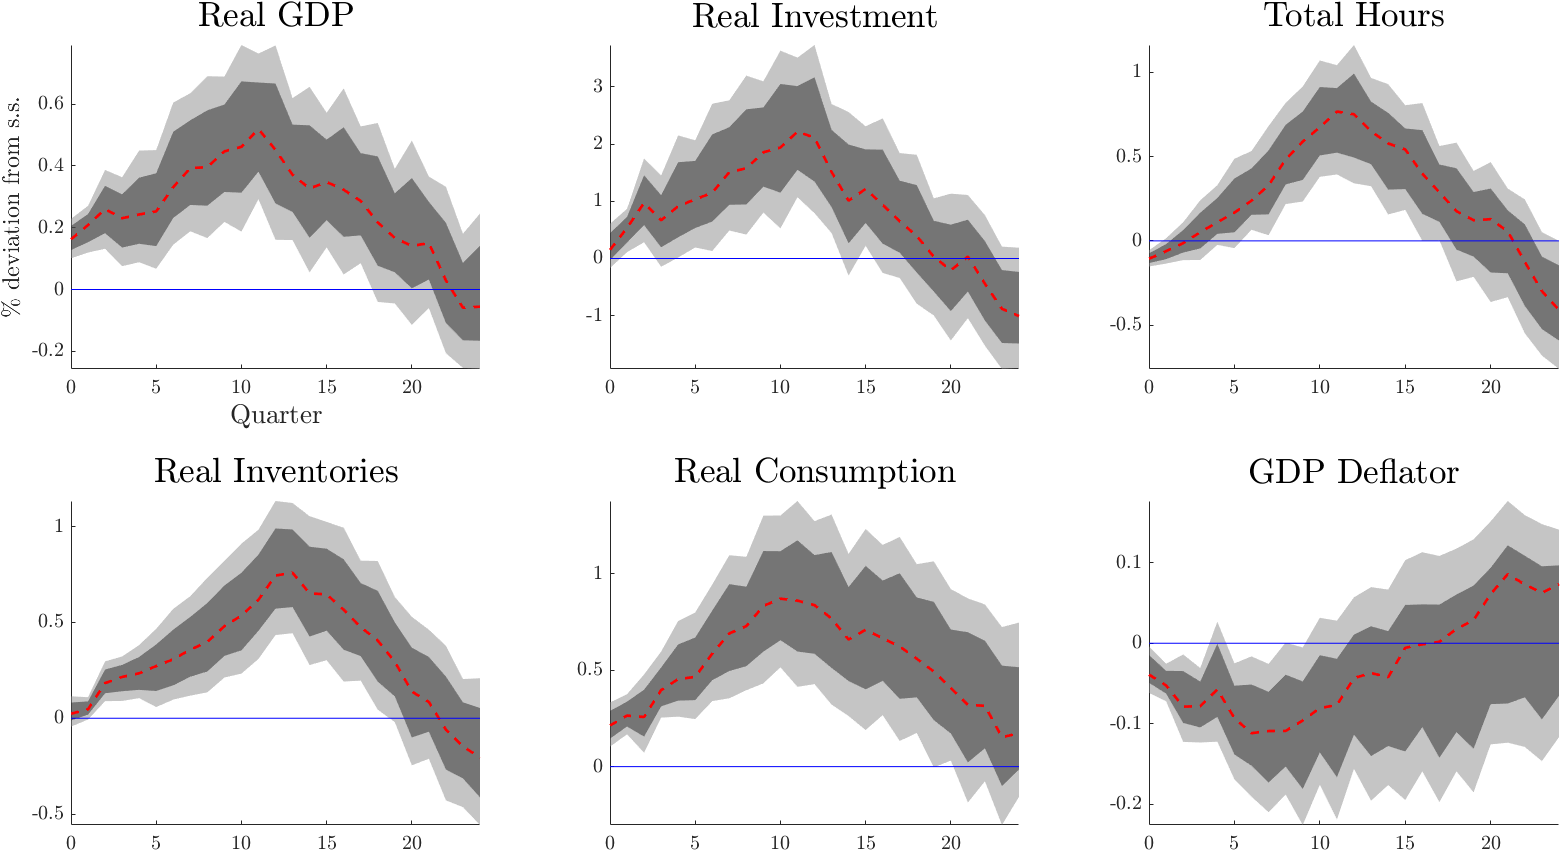
\includegraphics[scale=0.26]{tech_IRFs}
	
}


\end{document}